"Monte Carlo Policy Gradient Method for Binary Optimization"

In this paper, we consider the following binary optimization problem:
\begin{equation}
    \min _{x} \quad f(x), \quad \text { s.t. } \quad x \in \mathcal{B}_{n} \tag{1}
\end{equation}
where $\mathcal{B}_{n}=\{-1,1\}^{n}$ represents the binary set of dimension $n$ and $f$ can be any function defined on $\mathcal{B}_{n}$.

\section{2 Probabilistic Model for Binary Optimization}

\subsection{2.1 Parameterized Probabilistic Model}

The goal is to search for the set of (globally) optimal points $\mathcal{X}^{*}$ of (1) in the discrete space $\mathcal{B}_{n}$. A probabilistic approach is to consider an \textbf{indicator distribution}, i.e.,
\begin{equation}
    q^{*}(x)=\frac{1}{\left|\mathcal{X}^{*}\right|} \mathbb{1}_{\mathcal{X}^{*}}(x)= 
\begin{cases}\frac{1}{\left|\mathcal{X}^{*}\right|}, & x \in \mathcal{X}^{*}, \\ 0, & x \notin \mathcal{X}^{*}.
\end{cases}
\end{equation}
Here,
\begin{equation}
    \mathbb{1}_{\mathcal{X}}(x)= \begin{cases}1, & x \in \mathcal{X}^*, \\ 0, & x \notin \mathcal{X}^* .\end{cases}
\end{equation}
The distribution $q^{*}$ is the ideal distribution where only the optimal points have the uniform probability. If we sample according to $q^{*}$, then we will definitely get the optimal solution of (1). However, the optimal points set $\mathcal{X}^{*}$ is unknown. 

To approach $q^{*}$, we introduce the following family of \textbf{Gibbs distributions} with parameter $\lambda > 0$:
\begin{equation}
    q_{\lambda}(x)=\frac{1}{Z_{\lambda}} \exp \left(-\frac{f(x)}{\lambda}\right), \quad x \in \mathcal{B}_{n}, \tag{3}
\end{equation}
where $Z_{\lambda}=\sum_{x \in \mathcal{B}_{n}} \exp \left(-\frac{f(x)}{\lambda}\right)$ is the normalization factor. Given the (globally) optimal value $f^{*}$ of (1), for any $x \in \mathcal{B}_{n}$, we notice that
\begin{align}
q_{\lambda}(x) & =\frac{\exp \left(\frac{-f(x)}{\lambda}\right)}{\sum_{x \in \mathcal{B}_{n}} \exp \left(\frac{-f(x)}{\lambda}\right)} \\
& =\frac{\exp \left(\frac{f^{*}-f(x)}{\lambda}\right)}{\sum_{x \in \mathcal{B}_{n}} \exp \left(\frac{f^{*}-f(x)}{\lambda}\right)} \\
&=\frac{\exp \left(\frac{f^{*}-f(x)}{\lambda}\right)}{\left|\mathcal{X}^{*}\right|+\sum_{x \in \mathcal{B}_{n} / \mathcal{X}^{*}} \exp \left(\frac{f^{*}-f(x)}{\lambda}\right)}  \tag{4}\\
& \rightarrow q^{*}(x)=\frac{1}{\left|\mathcal{X}^{*}\right|} \mathbb{1}_{\mathcal{X}^{*}}(x), \quad \text { as } \lambda \rightarrow 0.
\end{align}
Note that the term in denominator, namely, $\sum_{x \in \mathcal{B}_n / \mathcal{X}^*} \exp \left(\frac{f^*-f(x)}{\lambda}\right) \to 0$ as $\lambda \to 0$. Although $q^{*}$ is not computable in practice, the Gibbs distribution $q_{\lambda}$, which converges to $q^{*}$ pointwisely, provides a feasible alternative for searching optimal solutions. In summary, for all points $x \in\mathcal{B}_n$, 
one has
\begin{equation}
    q_\lambda(x) \to q^*(x)=\frac{1}{\left|\mathcal{X}^*\right|} \mathbf{1}_{\mathcal{X}^*}(x), \quad \text { as } \lambda \rightarrow 0.
\end{equation}
\begin{remark}
    We had encoded the information of objective function $f$ of (1) into the probabilistic models, both $q^{*}$ without parameters and $q_\lambda$ with parameters $\lambda$.
\end{remark}

Motivated by this observation, one can devise an algorithm to randomly sample from the Gibbs distribution and control the parameter $\lambda$ to approximate the global optimum. 
\begin{enumerate}
    \item However, since $q_{\lambda}(x)$ needs to compute the summation of $2^{n}$ terms in the denominator $Z_{\lambda}$, the complexity of direct sampling grows exponentially.
    \item Meanwhile, $q_{\lambda}$ is hard to sample when $f$ owns a rough landscape.
\end{enumerate}

Instead of direct sampling from the Gibbs distribution, we approximate it using a parameterized policy distribution that can be sampled efficiently. 

Consider the problem instance $\mathcal{P}$, that is, a instance of objective $f$. For the moment, $\lambda >0$ is a constant that was set in advance. The parameterized \textit{policy distribution} $p_{\theta}(x \mid \mathcal{P})$ is designed to have a similar but regular landscape to that of $q_{\lambda}$ to enable efficient sampling. For notational convenience, we write
\begin{equation}
    p_{\theta}(x)=p_{\theta}(x \mid \mathcal{P}).
\end{equation}
(We shall give the concrete way to construct $p_{\theta}$ in next section.) To measure the distance between $p_{\theta}$ and $q_{\lambda}$, we introduce the \textbf{KL divergence} defined as follows:
\begin{equation}
    \mathrm{KL}\left(p_{\theta} \| q_{\lambda}\right)=\sum_{x \in \mathcal{B}_{n}} p_{\theta}(x) \log \frac{p_{\theta}(x)}{q_{\lambda}(x)}.
\end{equation}
In order to reduce the discrepancy between the policy distribution $p_{\theta}$ and the Gibbs distribution $q_{\lambda}$, we minimize this KL divergence with respect to the variable $\theta$. For the Gibbs distribution $q_\lambda$ in (3), we notice that
\begin{align}
\min _{\theta} \quad \mathrm{KL}\left(p_{\theta} \| q_{\lambda}\right) 
& =\sum_{x \in \mathcal{B}_{n}} p_{\theta}(x) \left( \log p_{\theta}(x) - \log q_{\lambda}(x) \right) \\
& =\sum_{x \in \mathcal{B}_{n}} p_{\theta}(x) \left( \log  p_{\theta}(x) - \log \left[ \frac{1}{Z_\lambda} \exp \left(-\frac{f(x)}{\lambda}\right) \right]\right)  \\
& =\sum_{x \in \mathcal{B}_{n}} p_{\theta}(x) \left( \log  p_{\theta}(x) - \log \frac{1}{Z_\lambda} + \frac{f(x)}{\lambda}\right) \\
& =\frac{1}{\lambda} \sum_{x \in \mathcal{B}_{n}} p_{\theta}(x) f(x)+\sum_{x \in \mathcal{B}_{n}} p_{\theta}(x) \log p_{\theta}(x)+\log Z_{\lambda} \\
& =\frac{1}{\lambda}\left(\mathbb{E}_{p_{\theta}}[f(x)]+\lambda \mathbb{E}_{p_{\theta}}\left[\log p_{\theta}(x)\right]\right)+\log Z_{\lambda} ,\tag{5}
\end{align} 
where we write 
\begin{equation}
    \mathbb{E}_{p_\theta}[f(x)] = \sum_{x \in \mathcal{B}_n} p_\theta(x) f(x)
\end{equation}
and
\begin{equation}
    \mathbb{E}_{p_\theta}\left[\log p_\theta(x)\right] = \sum_{x \in \mathcal{B}_n} p_\theta(x) \log p_\theta(x).
\end{equation}
Since $Z_{\lambda}$ is a constant, (5) is equivalent to the following problem:
\begin{equation}
    \min _{\theta} \quad L_{\lambda}(\theta)=\underbrace{\mathbb{E}_{p_{\theta}}[f(x)]}_{L(\theta)}+\lambda \underbrace{\mathbb{E}_{p_{\theta}}\left[\log p_{\theta}(x)\right]}_{H(\theta)} \tag{6}
\end{equation}
While minimizing (6) is to find an approximation of Gibbs distribution $q_{\lambda}$, one can explain (6) from the perspective of optimization. 

In (6), the first term $L(\theta)$ is the expected loss of $f(x)$ with $x \sim p_{\theta}$ and the second term $H(\theta)$ is the \textit{entropy regularization} of $p_{\theta}$. 
\begin{itemize}
    \item Minimizing the first term $L(\theta)$ yields the optimal value $f^{*}$ and $p_{\theta}\left(x \in \mathcal{X}^{*}\right)=1$. However, it leads to hardship on sampling as $p_{\theta}$ is rough. By adding the entropy regularization, we encourage exploration and promote the diversity of samples.
    \item On the other hand, the\textit{ regularization parameter} $\lambda$, which is also called \textit{annealing temperature}, progressively decreases from an initial positive value to zero as in the classical simulated annealing, and the global optimum are finally obtained after a sufficiently long time.
\end{itemize}

\subsection{2.2 Parameterization of Sampling Policy Distribution $p_{\theta}$}

As we discuss above, we can use probabilistic methods to solve binary optimization problems. 

The sampling policy can be parameterized by a neural network with $\mathcal{P}$ containing features of the problem, that is,
\begin{equation}
    p_{\theta}(x \mid \mathcal{P}) \propto e^{\phi_{\theta}(x, \mathcal{P})} \tag{7}
\end{equation}
where $\phi$ represents a neural network with input $x$ and problem instance $\mathcal{P}$. 

It is unrealistic to generate a normalized distribution over $2^{n}$ points in $\mathcal{B}_{n}$. The unnormalized policy (7) can be sampled through the Metropolis algorithm. The neural network can be designed to reduce the computational complexity in the sampling process. % 但是实验也没有用到neural network啊

One natural idea is to consider the distribution on each single variable (that is, each $x_{i} \in \{-1,+1\}$ in binary string $x=x_{1}x_{2}\dots x_{n}$ ) and assume independence, which is called the \textbf{mean field (MF) approximation} in statistical physics. 

The MF methods provide tractable approximations for the high dimensional computation in probabilistic models. By neglecting certain dependencies between random variables, we simplify the parameterized distribution $p_{\theta}$ with the independent assumption for each component of $x$. As for binary optimization problems $\mathcal{P}$ in (1), the parameterized probability follows the \textit{multivariate Bernoulli distribution}:
\begin{equation}
    p_{\theta}(x)=\prod_{i=1}^{n} \mu_{i}^{\left(1+x_{i}\right) / 2}\left(1-\mu_{i}\right)^{\left(1-x_{i}\right) / 2}, \quad \mu_{i}=\operatorname{sigmoid}(x_i)=\frac{1}{1+e^{-\theta_{i}}}, \tag{8}
\end{equation}
where $\theta_{i}, i=1, \ldots, n$ are parameters. Under the mean field approximation, $x_{1}, x_{2}, \ldots, x_{n}$ are viewed independent and $\mu_{i}$ is the probability that the $i$-th variable $x_{i}$ takes value "+1". Note that $\left(1+x_{i}\right)/2=1$ and $\left(1-x_{i}\right)/2=0$ for $x_i = +1$; on the other hand, $\left(1+x_{i}\right)/2=0$ and $\left(1-x_{i}\right)/2=1$ for $x_i = -1$.

The MF approximation provides an efficient way to encode binary optimization problems and greatly reduces the complexity of the model from $2^{n}$ to $n$. Besides, the distribution under MF approximation is beneficial for the Markov chain Monte Carlo sampling. %  encode binary optimization problems, 这里唯一编码了问题的可行解,即binary特征,而和f无关。

\subsection{2.3 Prototype Algorithm}

In the above discussion, we have already constructed the loss function $L_{\lambda}(\theta)$ and a mean field sampling policy $p_{\theta}(x)$. Sometimes, we often only say "policy", or "sampling policy" for the short of "sampling policy distribution $p_{\theta}$".

To train the policy, the gradient formulation is derived explicitly in following Lemma 1. Then, we purpose the brief algorithm framework. The sampled solutions help to compute the policy gradient and improve the sampling policy. The policy is optimized by the stochastic policy gradient, which guides us to sample those points with lower function values. Thus, the binary optimization problems are solved by stochastic sampling based on a neural network policy. % neural network policy 怎么又出现了nn?有没有用到。

\begin{lemma}[Lemma 1]
    Suppose for any $x \in \mathcal{B}_{n}$, the policy $p_{\theta}(x)$ is differentiable with respect to $\theta$. For any constant $c \in \mathbb{R}$, the gradient of the loss function (6) is given by
\begin{equation}
    \nabla_{\theta} L_{\lambda}(\theta)=\mathbb{E}_{p_{\theta}}\left[\left(f(x)+\lambda \log p_{\theta}(x)-c\right) \nabla_{\theta} \log p_{\theta}(x)\right]. \tag{9}
\end{equation}
This gradient is called the policy gradient.
\end{lemma}
\begin{proof}
    By exchanging the order of differentiation ($\nabla$ operations) and summation, we note that
\begin{align}
\mathbb{E}_{p_{\theta}}\left[\nabla_{\theta} \log p_{\theta}(x)\right]
&=\mathbb{E}_{p_{\theta}}\left[ \frac{1}{p_{\theta}(x)}\nabla_{\theta} p_{\theta}(x)\right] \\
&=\sum_{x \in \mathcal{B}_{n}} p_{\theta}(x) \cdot \frac{1}{p_{\theta}(x)}\nabla_{\theta} p_{\theta}(x)\\
&=\sum_{x \in \mathcal{B}_{n}} \nabla_{\theta} p_{\theta}(x) \\
&=\nabla_{\theta} \sum_{x \in \mathcal{B}_{n}} p_{\theta}(x) \\
&=\nabla_{\theta} 1=0 \tag{10}
\end{align}
as $\sum_{x \in \mathcal{B}_{n}} p_{\theta}(x)=1$ is a constant. The gradient of the loss function (6) 
\begin{align}
    L_{\lambda}(\theta) &= \sum_{x \in \mathcal{B}_n} p_\theta(x) f(x)+ \lambda \sum_{x \in \mathcal{B}_n} p_\theta(x) \log p_\theta(x) \\
    & = \sum_{x \in \mathcal{B}_n} p_\theta(x)\left(f(x)+\lambda \log p_\theta(x)\right).
\end{align}
is derived by
\begin{equation}
\begin{aligned}
\nabla_{\theta} L_{\lambda}(\theta) & =\nabla_{\theta} \sum_{x \in \mathcal{B}_{n}} p_{\theta}(x)\left(f(x)+\lambda \log p_{\theta}(x)\right) \\
& =\lambda \sum_{x \in \mathcal{B}_{n}} p_{\theta}(x) \nabla_{\theta} \log p_{\theta}(x)+\sum_{x \in \mathcal{B}_{n}}\left(f(x)+\lambda \log p_{\theta}(x)\right) \nabla p_{\theta}(x) \\
& \stackrel{(i)}{=} \lambda \sum_{x \in \mathcal{B}_{n}} \nabla_{\theta} p_{\theta}(x)+\sum_{x \in \mathcal{B}}\left(f(x)+\lambda \log p_{\theta}(x)\right) p_{\theta}(x) \nabla_{\theta} \log p_{\theta}(x) \\
& \stackrel{(i i)}{=} \sum_{x \in \mathcal{B}} p_{\theta}(x) \left(f(x)+\lambda \log p_{\theta}(x)\right)  \nabla_{\theta} \log p_{\theta}(x) \\
& =\mathbb{E}_{p_{\theta}}\left[\left(f(x)+\lambda \log p_{\theta}(x)\right) \nabla_{\theta} \log p_{\theta}(x)\right]
\end{aligned}
\end{equation}

where ( $i$ ) uses the substitution 
\begin{equation}
    \nabla_{\theta} p_{\theta}(x)=p_{\theta}(x) \cdot \nabla_{\theta} \log p_{\theta}(x)
\end{equation}
and (ii) is due to (10). For any given $c$ irrelevant to $x,(10)$ yields that $\mathbb{E}_{p_{\theta}}\left[c \nabla_{\theta} \log p_{\theta}(x)\right]=0$. This completes the proof.
\end{proof}

Especially, we take % c 是依赖于theta的值,可以这么取常数c吗?
\begin{equation}
    c=\mathbb{E}_{p_{\theta}}[f(x)]
\end{equation}
and denote 
\begin{equation}
    A_{\lambda}(x ; \theta)=f(x)+\lambda \log p_{\theta}(x)- \mathbb{E}_{p_{\theta}}[f(x)].
\end{equation}
In this case, the policy gradient is 
\begin{equation}
    \nabla_\theta L_\lambda(\theta)=\mathbb{E}_{p_\theta}\left[ A_{\lambda}(x ; \theta) \cdot \nabla_\theta \log p_\theta(x)\right].
\end{equation}
We call the function $A_{\lambda}(x ; \theta)$ as the "\textbf{advantage function}" analogous to the one in reinforcement learning [40]. It has been shown that such technique can reduce the variance in our training and make it easier to sample points with lower cost. 

Hence, the stochastic gradient is computed by
\begin{equation}
\begin{aligned}
A_{\lambda}(x ; \theta, S) & =f(x)+\lambda \log p_{\theta}(x)-\sum_{x \in S} f(x), \\
\bar{g}(\theta, S) & =\sum_{x \in S} A_{\lambda}(x ; \theta, S) \nabla_{\theta} \log p_{\theta}(x).
\end{aligned}
\end{equation}
where $S$ is a sample set from the distribution $p_{\theta}(x)$.

Finally, we propose a prototype algorithm for solving binary optimization problems as follows:

\begin{enumerate}
    \item At the beginning of each iteration, the probabilistic model provides a distribution $p_{\theta}(\cdot \mid \mathcal{P})$, indicating where the good solution potentially lies.
    \item A set of points $S$ are sampled from $p_{\theta}(\cdot \mid \mathcal{P})$.
    \item The policy gradient is computed in order to update the probabilistic model, providing an improved distribution for the next iteration.
    \item The parameter $\theta$ in the probabilistic model is updated as follows
  \begin{equation}
    \theta^{t+1}=\theta^{t}-\eta^{t} \bar{g}\left(\theta^{t}, S^{t}\right)
\end{equation}
  where $\eta^{t}$ and $S^{t}$ are the step size and the sample set at the $t$-th iteration.
\end{enumerate}

Algorithm 1 gives the pseudo-code of the prototype algorithm. 
\begin{figure}
    \centering
    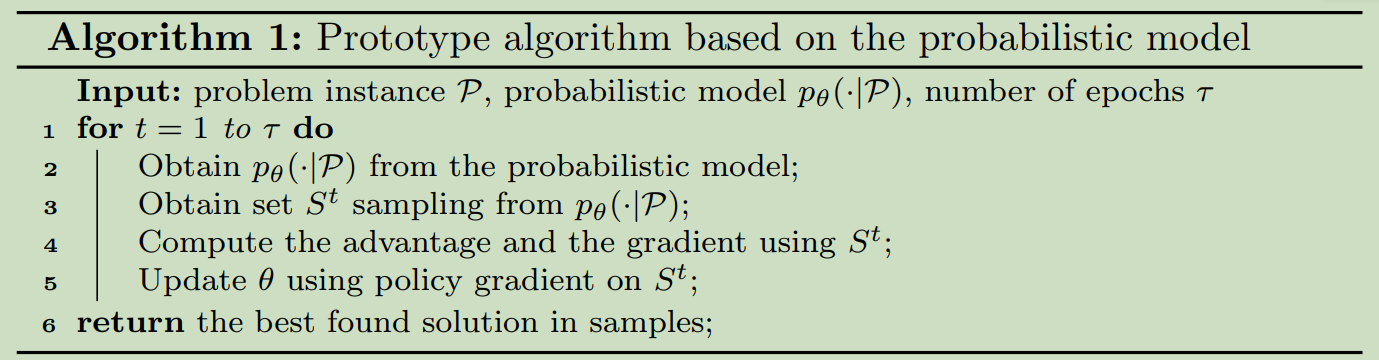
\includegraphics[width=1\linewidth]{Images/MCPG_ALG_1.png}
\end{figure}
The prototype algorithm is efficient in obtaining better solutions compared to most naive heuristic methods, since similar frameworks are commonly used in machine learning. However, it also faces several critical challenges. 
\begin{itemize}
    \item It is difficult to determine whether a good solution has been achieved.
    \item Moreover, keeping the diversity of samples remains challenges at the later iterations. On the other hand, due to the NP-hard nature of the problem (1), there are many local minimum in solving problem (6), making it challenging for policy gradient methods to find global minima. This difficulty is prevalent in most reinforcement learning scenarios.
\end{itemize}

\section{3 A Monte Carlo Policy Gradient Method} %至此,我们没有解释具体如何根据p_theta采样得到S,本节的3.1,3.2的算法的目的就是详述采样的一个好办法。可以直接跳到3.3节看整体。

\begin{figure}
    \centering
    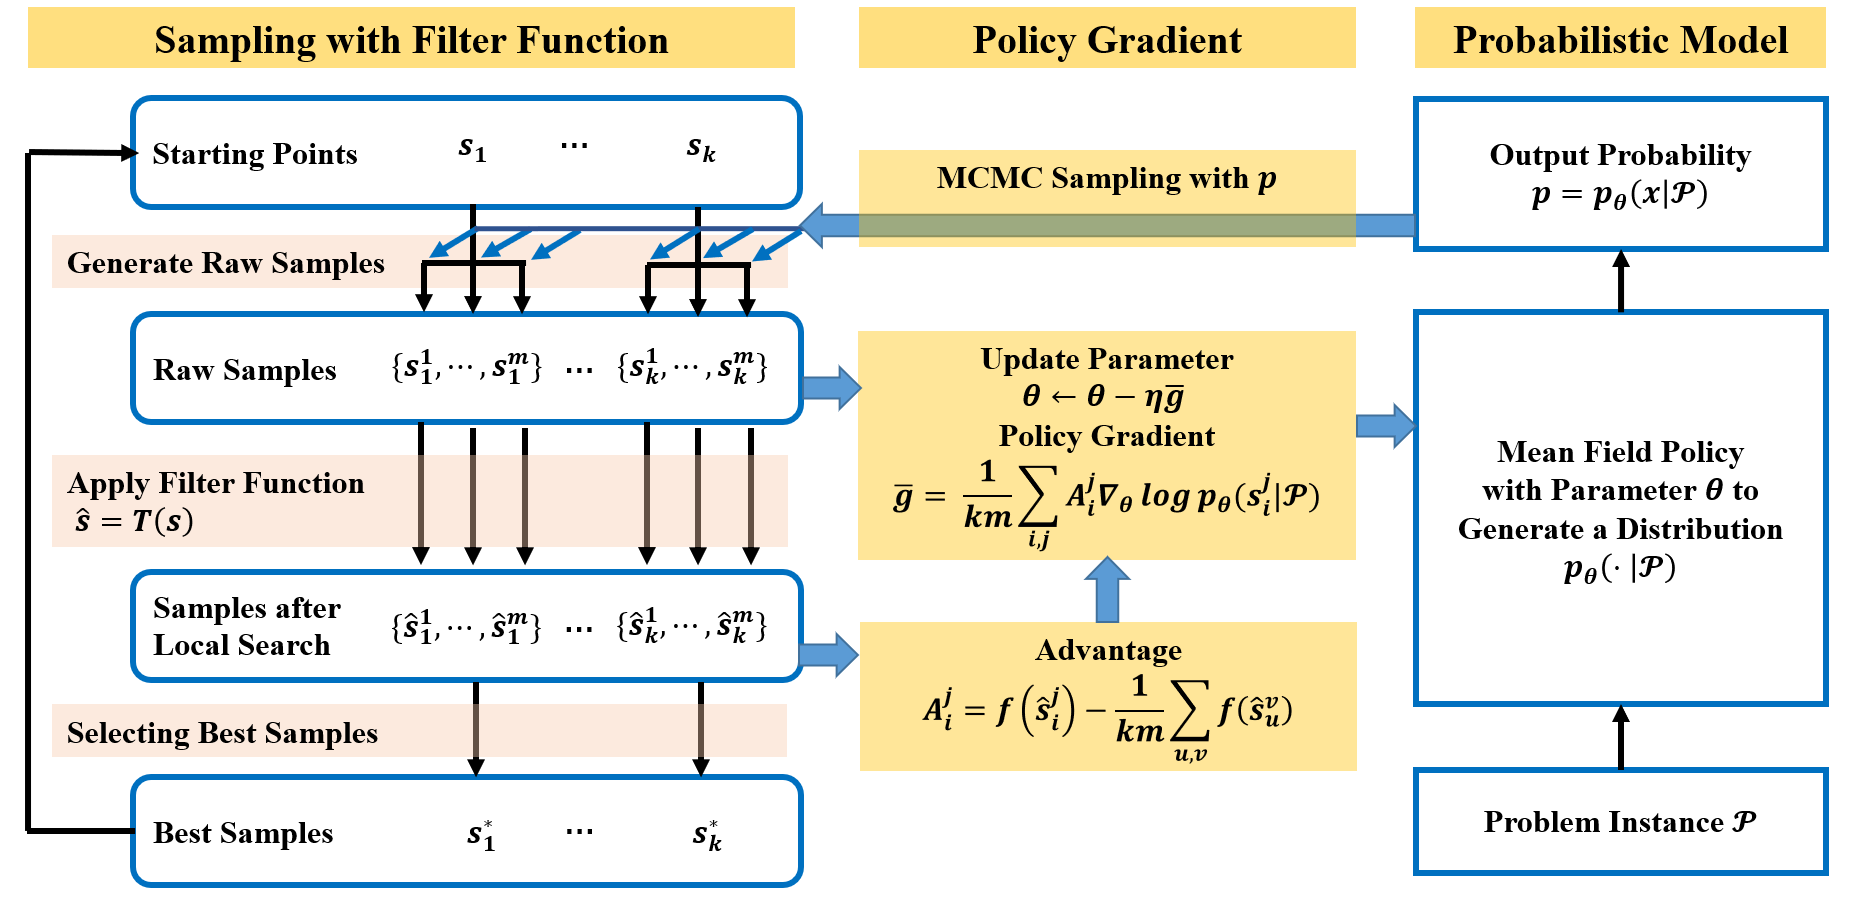
\includegraphics[width=1\linewidth]{Images/MCPG_pipeline.png}
    \caption{Enter Caption}
    \label{fig:enter-label}
\end{figure}

\begin{figure}
    \centering
    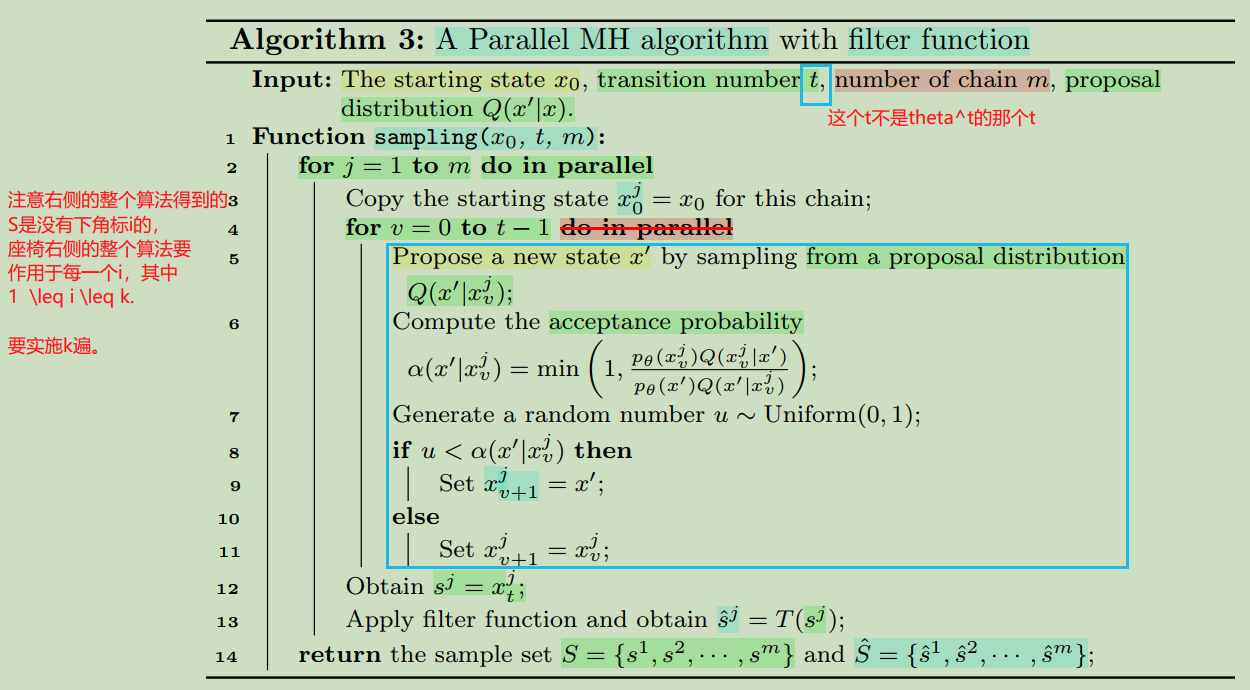
\includegraphics[width=1\linewidth]{Images/MCPG_ALG_3.png}
\end{figure}

\begin{figure}
    \centering
    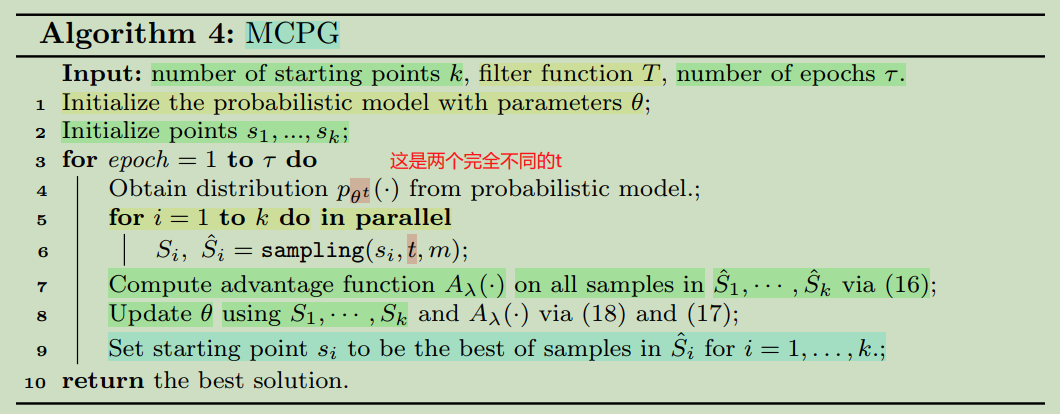
\includegraphics[width=1\linewidth]{Images/MCPG-ALG-4.png}
\end{figure}

